\documentclass[preprint]{article}

\PassOptionsToPackage{numbers,compress}{natbib}

\usepackage[]{neurips_2021}
\usepackage[utf8]{inputenc} 
\usepackage[T1]{fontenc}    
\usepackage{hyperref}       
\usepackage{url}            
\usepackage{booktabs}       
\usepackage{nicefrac}       
\usepackage{microtype}      
\usepackage{amsfonts,amsmath,amssymb}	
\usepackage{mathtools}
\usepackage{lipsum}
\usepackage[dvipsnames]{xcolor}

\definecolor{linkcolor}{rgb}{0.7752941176470588, 0.22078431372549023, 0.2262745098039215}
\hypersetup{colorlinks=true,
linkcolor=linkcolor,
citecolor=linkcolor,
urlcolor=linkcolor,
linktocpage=true,
pdfproducer=medialab,
}

\title{Inferring dark matter substructure with \\ astrometric lensing beyond the power spectrum}

\author{
Siddharth Mishra-Sharma \\
The NSF AI Institute for Artificial Intelligence and Fundamental Interactions \\
Massachusetts Institute of Technology \\
Harvard University \\ 
New York University \\
\href{mailto:smsharma@mit.edu}{\texttt{smsharma@mit.edu}} \\
}

\begin{document}

\hfill MIT-CTP/5331
\maketitle

\begin{abstract}
Astrometry---the precise measurement of positions and motions of celestial objects---has recently emerged as a promising avenue for characterizing the dark matter population in our Galaxy. By leveraging recent advances in simulation-based inference and neural network architectures, we introduce a novel method to search for a global dark matter-induced gravitational lensing signature in astrometric datasets. Our method based on neural likelihood-ratio estimation shows significantly enhanced sensitivity to a cold dark matter population and more favorable scaling with measurement noise compared to existing approaches based on two-point correlation statistics, establishing machine learning as a powerful tool for characterizing dark matter using astrometric data. 
\end{abstract}

\section{Introduction and background}
\label{sec:intro}

Although there exists plenty of evidence for dark matter (DM) on galactic scales and above (see Ref.~\cite{Green:2021jrr} for a recent overview), the distribution of DM clumps---subhalos---on sub-galactic scales is less well-understood and remains an active area of cosmological study. This distribution additionally correlates with and may provide clues about the underlying particle physics nature of dark matter (see \emph{e.g.}, Refs.~\cite{Schutz:2020jox,Bode:2000gq,Dalcanton:2000hn}), highlighting its relevance across multiple domains.

While more massive dark matter subhalos can be detected and studied through their association with luminous tracers such as bound stellar populations, subhalos with smaller masses $\lesssim 10^9\,\mathrm M_\odot$ are not generally associated with luminous matter~\cite{Fitts:2016usl,2017MNRAS.467.2019R}, rendering their characterization challenging. Gravitational effects provide one of the few avenues to probe the distribution of these otherwise-invisible subhalos~\cite{Buckley:2017ijx}. Gravitational lensing \emph{i.e.}, the bending of light from a background source due to a foreground mass, is one such effect and has been proposed in various incarnations as a probe of dark subhalos. 
Strong gravitational lensing, for example, has been used to infer the presence of dark matter substructure in galaxies outside of our own~\cite{Hezaveh:2016ltk,Vegetti:2009cz,Gilman:2019nap,Vegetti:2012mc}.
Astrometric lensing, on the other hand, has recently emerged as a promising way to characterize the dark matter subhalo population in the Milky Way.

Astrometry refers to the precise measurement of the positions and motions of luminous objects like stars and galaxies. Gravitational lensing of these background objects by a moving foreground mass, such as a dark matter subhalo, can imprint a characteristic, correlated pattern on their measured kinematics (angular velocities and/or accelerations). Ref.~\cite{VanTilburg:2018ykj} introduced several methods for extracting this signature with the aim of characterizing the subhalo population in our Galaxy, including those based on computing convolutions of the expected lensing signal on astrometric datasets and detecting local kinematic outliers. Ref.~\cite{Mondino:2020rkn} applied the former method to data from the \emph{Gaia} satellite, obtaining constraints on the abundance of dark compact objects in the Milky Way and showcasing the applicability of astrometric dark matter searches in a practical setting. Finally, Ref.~\cite{Mishra-Sharma:2020ynk} proposed using the angular power spectrum of the astrometric field as an observable to infer the population properties of Galactic dark matter, leveraging the collective, correlated signal of a large subhalo sample. 

Astrometric datasets are inherently high-dimensional, consisting of positions and kinematics of potentially millions of objects. Especially when the expected signal consists of the collective imprint of a large number of lenses, characterizing their population properties involves marginalizing over all possible configurations of subhalos, rendering the likelihood intractable and usually necessitating the use of simplified data representations like the power spectrum. While effective, such simplification can result in loss of information when the signal is non-Gaussian in nature. The existence of systematic effects that are degenerate with a putative signal in the low-dimensional summary domain can further inhibit sensitivity. 

The dawn of the era of precision astrometry, with the \emph{Gaia} satellite~\cite{2016A&A...595A...1G} having recently delivered the most precise astrometric dataset to-date~\cite{2018A&A...616A...1G,2018A&A...616A...2L,2021A&A...649A...1G} and surveys including the Square Kilometer Array (SKA)~\cite{Fomalont:2004hr,Jarvis:2015tqa} and Roman Space Telescope~\cite{2019JATIS...5d4005W} set to achieve further leaps in sensitivity over the next decade, calls for methods that can extract more information from these datasets than is possible using existing techniques. In this paper we introduce such a method that uses spherical convolutional neural networks in conjunction with parameterized classifiers~\cite{Cranmer:2015bka,Baldi:2016fzo} in order to estimate likelihood ratios associated with the abundance of a cold dark matter population directly from a binned map of the astrometric velocity field. 
We show that our method outperforms established proposals based on the two-point correlation statistics of the astrometric field, both in absolute sensitivity as well as in the scaling of projected uncertainty with measurement noise.

\section{Model and inference}
\label{sec:model}

\begin{figure}[!htbp]
\centering
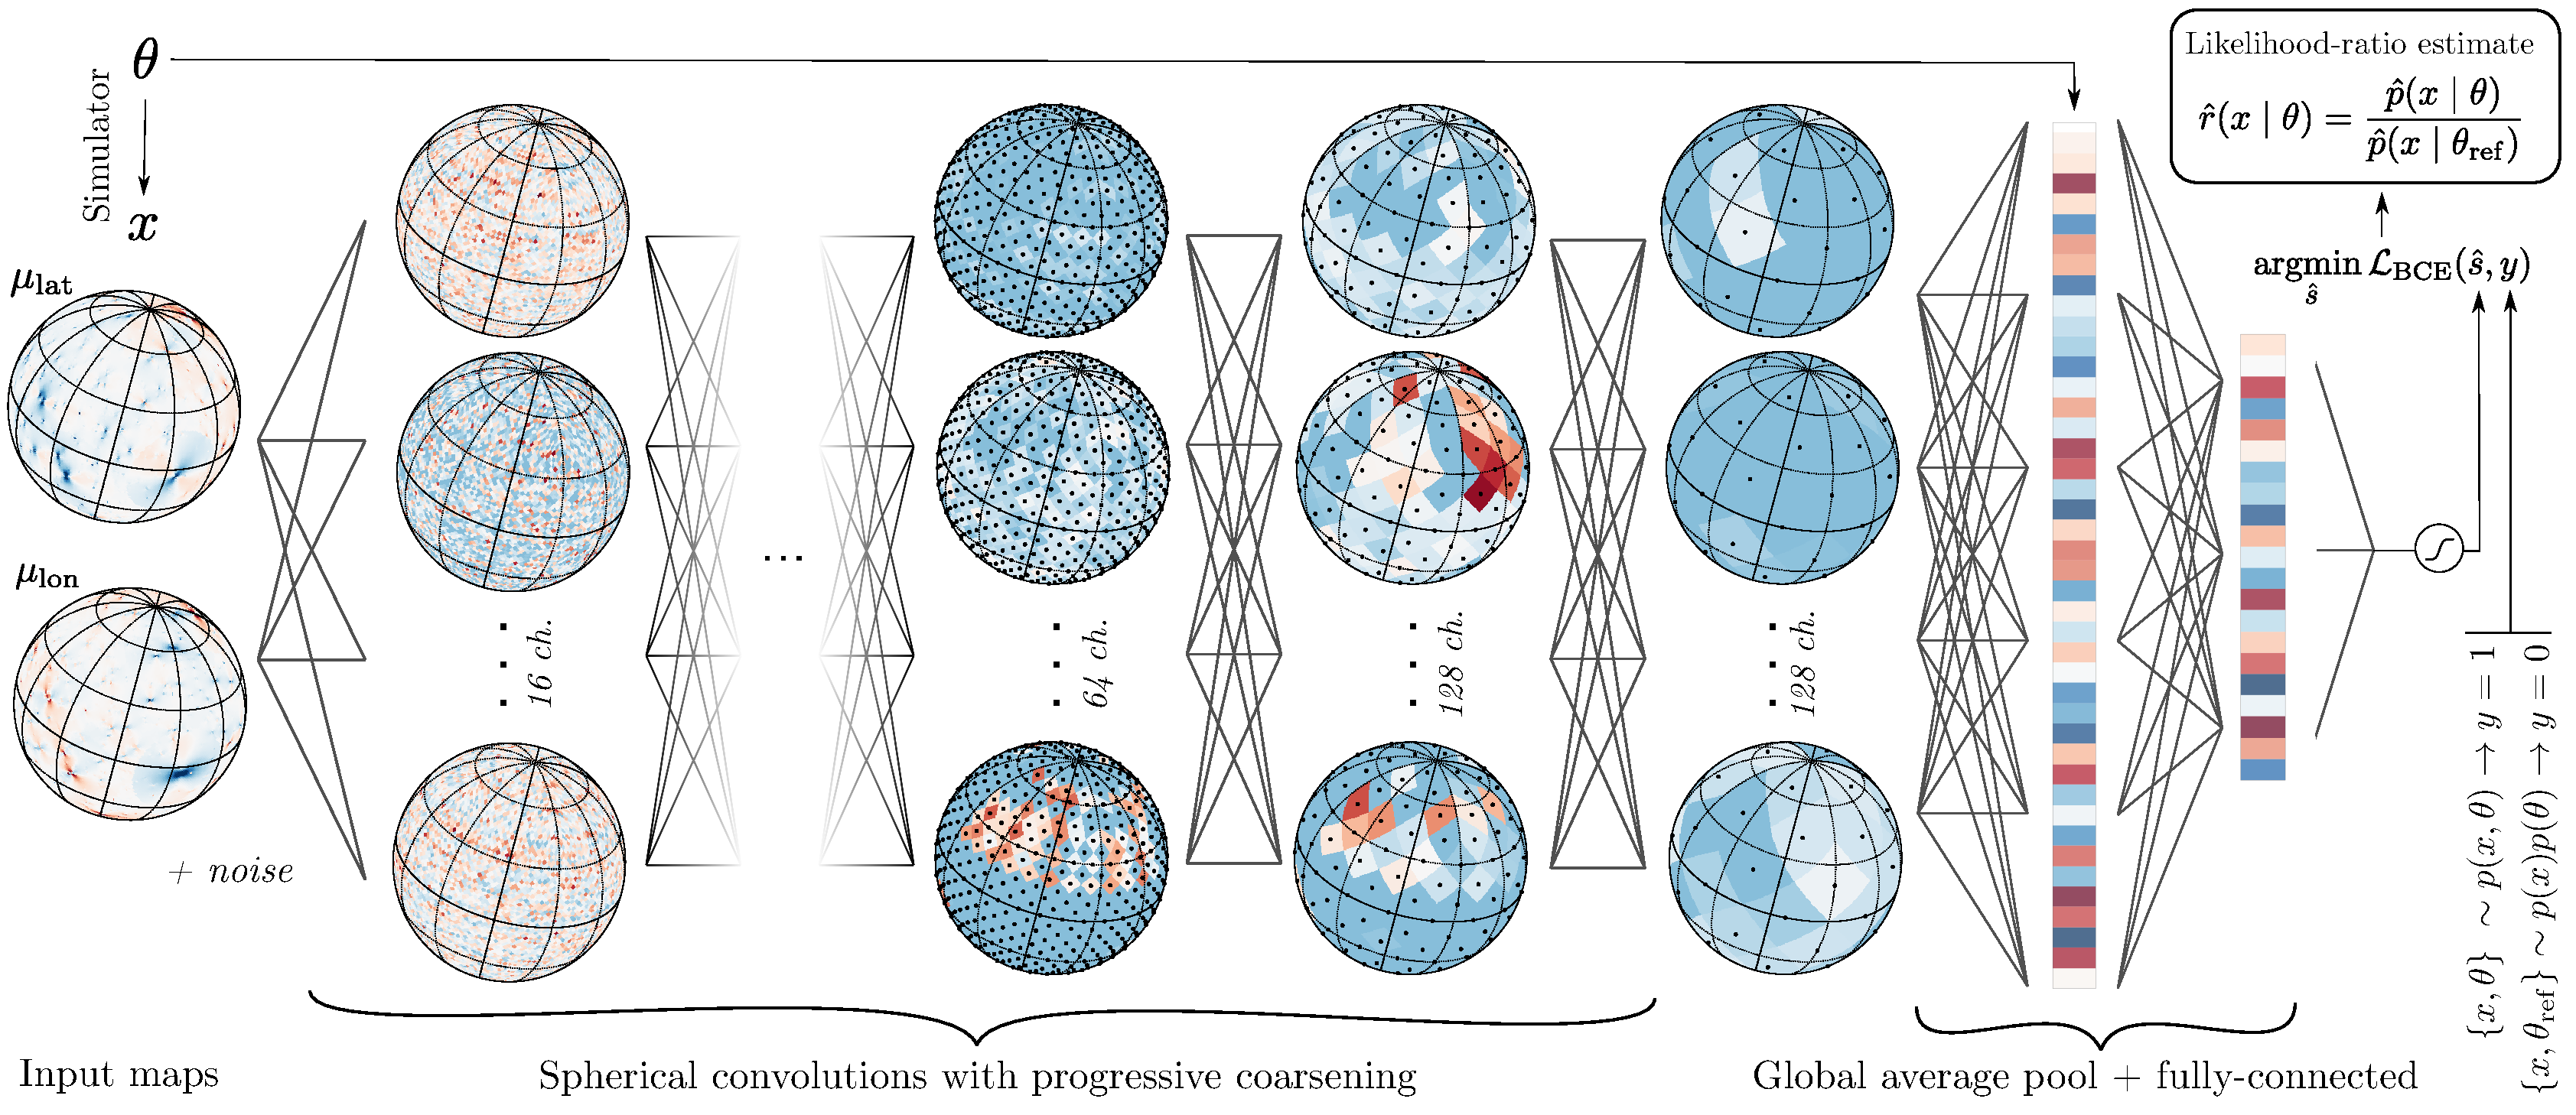
\includegraphics[width=1.00\textwidth]{figures/drawing.pdf}
\caption{An illustration of the method and neural network architecture used in this work.}
\label{fig:model}
\end{figure}

\paragraph{The forward model} We consider a population of Navarro-Frenk-White (NFW)~\cite{Navarro:1995iw} subhalos following a power-law mass function, $\mathrm dn / \mathrm dm \propto m^\alpha$, with slope $\alpha = -1.9$ as expected if the population is sourced from nearly scale-invariant primordial fluctuations in the canonical $\Lambda$ Cold Dark Matter ($\Lambda$CDM) scenario. The concentration-mass relation from Ref.~\cite{Sanchez-Conde:2013yxa} is used to model the concentrations associated with density profiles of individual subhalos. 

Subhalos between $10^7$--$10^{10}\,\mathrm{M}_\odot$ are simulated, assuming the influence of lighter subhalos to be too small to be discernable~\cite{Mishra-Sharma:2020ynk}. The subhalo fraction $f_\mathrm{sub}$, quantifying the expected fraction of the mass of the Milky Way contributed by subhalos in the range $10^{-6}$--$10^{10}\,\mathrm{M}_\odot$, is taken to be the parameter of interest. The spatial distribution of subhalos in the Galactocentric frame is modeled using results from the Aquarius simulation following Refs.~\cite{Hutten:2016jko,Springel:2008cc}. Since this spatial distribution accounts for the depletion of subhalos towards the Galactic Center due to gravitational tidal effects, the angular number density of subhalos looking out from the Sun frame can be considered to be effectively isotropic.

A truncated Maxwellian $f_{\infty}(\mathbf{v})\propto e^{-\mathbf{v}^{2} / v_{0}^{2}}\cdot H(v_\mathrm{esc} - |\mathbf{v}|)$ is used to model the asymptotic velocity distribution of subhalos in the Galactocentric frame~\cite{1939isss.book.....C,Lisanti:2016jxe}, where $v_\mathrm{esc}$ is the Galactic escape velocity and $H$ the Heaviside step function; see Ref.~\cite{Mishra-Sharma:2020ynk} for further details. A Galilean boost $f_{\odot}(\mathbf{v}) \approx f_{\infty}\left(\mathbf{v}+\mathbf{v}_{\odot}\right)$ is used to transform the velocities into the Sun frame, where $\mathbf{v}_{\odot} = (11, 232, 7)\,\mathrm{km}\,\mathrm{s}^{-1}$ is the Galactocentric velocity of the Sun. Note that the asymmetry in the direction of motion of the Sun in the Milky Way introduces a preferred direction for the Sun-frame velocities of subhalos, breaking strict rotation invariance in the forward model. Although not pursued here, this asymmetry can be used as an additional distinguishing handle for the lensing signal.

Our datasets consist of the 2-dimensional angular velocity map of background sources on the celestial sphere. We assume the sources to be isotropically distributed, although this assumption can be easily relaxed for a realistic source population.
Given a spherically-symmetric subhalo lens moving with transverse velocity $\mathbf{v}_{l}$, the expected lens-induced velocity for a quasar at impact parameter $\mathbf{b}$ is given by~\cite{VanTilburg:2018ykj}
\begin{equation}
    \boldsymbol{\mu}(\mathbf{b})=4 G_{\mathrm{N}}\left\{\frac{M(b)}{b^{2}}\left[2 \hat{\mathbf{b}}\left(\hat{\mathbf{b}} \cdot \mathbf{v}_{l}\right)-\mathbf{v}_{l}\right]-\frac{M^{\prime}(b)}{b} \hat{\mathbf{b}}\left(\hat{\mathbf{b}} \cdot \mathbf{v}_{l}\right)\right\}
\end{equation}
where $M(b)$ and $M^{\prime}(b)$ are the projected mass of the subhalo at a given impact parameter and its gradient. An example of the induced velocity signal on part of the celestial sphere, projected along the Galactic latitudinal and longitudinal directions and exhibiting dipole-like structures, is shown in the leftmost column of Fig.~\ref{fig:model}.

We take our source population to consist of remote, point-like galaxies known as quasars which, due to their large distances from the Earth, are not expected to have significant intrinsic angular velocities. In order to enable a comparison with traditional approaches---which are generally not expected to be sensitive to a cold dark matter subhalo population with next-generation astrometric surveys~\cite{VanTilburg:2018ykj,Mishra-Sharma:2020ynk}---we benchmark using an optimistic observational configuration corresponding to measuring the proper motions of $N_q = 10^8$ quasars with noise $\sigma_{\mu} = 0.1\,\mu\mathrm{as}\,\mathrm{yr}^{-1}$.

\paragraph{The power spectrum approach} Ref.~\cite{Mishra-Sharma:2020ynk} introduced an approach for extracting the astrometric signal due to a dark matter subhalo population by decomposing the observed map into its angular (vector) power spectrum. The power spectrum is a summary statistic ubiquitous in astrophysics and cosmology and quantifies the amount of correlation contained at different spatial scales. In the case of data on a sphere, the basis of spherical harmonics is often used, and the power spectrum then encodes the correlation structure on different multipoles $\ell$. The power spectrum effectively captures the linear component of the signal and, when the underlying signal is a Gaussian random field, captures \emph{all} of the relevant information contained in the map(s)~\cite{Tegmark:1996qt}.
The expected signal in the power spectrum domain can be computed semi-analytically using the formalism described in Ref.~\cite{Mishra-Sharma:2020ynk} and, given a noise model and assuming a Gaussian likelihood, the expected sensitivity can be computed using a Fisher forecast. We use this prescription as a comparison point to the method introduced here.

While effective, reduction of the full astrometric map to its power spectrum results in loss of information; this can be seen from the fact that the signal in the leftmost column of Fig.~\ref{fig:model} is far from Gaussian. Furthermore, the existence of correlations on large angular scales due to \emph{e.g.}, biases in calibration of celestial reference frames~\cite{2018A&A...616A..14G} or systematic variations in measurements taken over different regions of the sky introduces degeneracies with a putative signal and precludes their usage in the present context. For this reason multipoles $\ell < 10$ were discarded in Ref.~\cite{Mishra-Sharma:2020ynk}, degrading the projected sensitivity.

\paragraph{Likelihood-ratio estimation using parameterized classifiers} Recent advances in machine learning have enabled methods that aim to directly extract useful representations from models defined through high-dimensional simulations; see Ref.~\cite{Cranmer:2019eaq} for a recent review. Here, we make use of parameterized classifiers~\cite{Cranmer:2015bka,Baldi:2016fzo,Brehmer:2018eca,Brehmer:2018hga,Brehmer:2018kdj,Hermans:2019ioj} (previously used in Refs.~\cite{Brehmer:2019jyt,Hermans:2020skz} in the context of inferring DM substructure) in order to directly approximate the likelihood ratios associated with all-sky astrometric maps containing signatures of dark matter. Given a classifier that can distinguish between samples $\{x\} \sim p(x\mid\theta)$ drawn from parameter points $\theta$ and those from a fixed reference hypothesis $\{x\} \sim p(x\mid\theta_\mathrm{ref})$, the decision function output by the optimal classifier $s(x, \theta) = {p(x\mid\theta)}/{\left(p(x\mid\theta) + p(x\mid\theta_\mathrm{ref})\right)}$ is one-to-one with the likelihood ratio, $r(x\mid \theta) \equiv {p(x\mid\theta)}/{p(x\mid\theta_\mathrm{ref})}  = {s(x, \theta)}/{\left(1 - s(x, \theta)\right)}$, a fact appreciated as the likelihood-ratio trick~\cite{Cranmer:2015bka,mohamed2017learning}. 

The classifier $s(x, \theta)$ in this case is a neural network that can work directly on the high-dimensional data $x$, and is parameterized by $\theta$ by having it included as a feature. In order to improve numerical stability and reduce dependence on the fixed reference hypothesis $\theta_\mathrm{ref}$, we follow Ref.~\cite{Hermans:2019ioj} and train a classifier to distinguish between data-sample pairs $\{x, \theta\} \sim p(x,\theta)$ and those from a product of marginal distributions $\{x, \theta\} \sim p(x)p(\theta)$ (in practice obtained by shuffling samples within a batch) using the binary cross-entropy (BCE) loss as the optimization objective. 

\paragraph{Extracting information from high-dimensional astrometric maps} We bin the the velocity maps on a \texttt{HEALPix} grid~\cite{Gorski:2004by} with resolution parameter \texttt{nside=64}, corresponding to 49,152 pixels over the full sky with pixel area $\sim 0.8\,\mathrm{deg}^2$. The values within each pixel then quantify the average latitudinal and longitudinal velocity components of quasars within that pixel. All inputs are respectively normalized to zero mean and unit standard deviation across the training sample. 

We use \texttt{DeepSphere}~\cite{defferrard2020deepsphere,Perraudin:2018rbt}, a graph-based convolutional neural network architecture tailored to data sampled on a sphere and able to leverage the hierarchical structure of the \texttt{HEALPix} representation. In particular, \texttt{DeepSphere} efficiently performs convolutions in the spectral domain, using a basis of Chebychev polynomials as convolutional kernels~\cite{defferrard2016convolutional}; here, we set $K=4$ as the maximum polynomial order. Starting with 2 scalar input channels representing the two orthogonal (Galactic latitude and longitude) components of the velocity vector, we perform a graph convolution operation, increasing the channel dimension to 16 followed by a batch normalization, ReLU nonlinearity, and downsampling the representation by a factor of 4 with max pooling into the next coarser \texttt{HEALPix} representation. Pooling leverages scale separation, preserving important characteristics of the signal across different resolutions. 
Four more such layers are employed, increasing the channel dimension by a factor of 2 at each step until a maximum of 128, with the final map having resolution \texttt{nside=2} corresponding to 48 pixels. At this stage, we average over the spatial dimension (known as global average pooling~\cite{lin2014network}) in order to encourage approximate rotation invariance\footnote{We note that by representing the input angular velocity vector field in terms of two input scalar channels, we break the desired rotation equivariance of spherical convolutions due to differences in how scalar and vector representations transform under rotations. Although this will have a downstream effect on rotation invariance, a detailed study of how this influences the performance of our model is beyond the scope of this paper.}, outputting 128 features onto which the parameter of interest $f_\mathrm{sub}$ is appended. This is passed through a fully-connected network with (1024, 128) hidden units and ReLU activations outputting the classifier decision $\hat s$ by applying a sigmoidal projection.

\bigskip

$10^5$ maps from the forward model were produced, with 15\% of these held out for validation. The estimator was trained using a batch size of 64 for up to 50 epochs with early stopping if the validation loss had not improved after 10 epochs. The \texttt{Adam} optimizer~\cite{kingma2017adam} was used with initial learning rate $10^{-3}$ decayed through cosine annealing. A coarse grid search was used to inform the architecture choices and hyperparameters. 
Figure~\ref{fig:model} summarizes the neural network architecture and method used in this work.

% LRT~\cite{Cranmer:2015bka}
% AALR~\cite{Hermans:2019ioj}
% SBI~\cite{Cranmer:2019eaq}

\begin{figure}[!htbp]
\centering
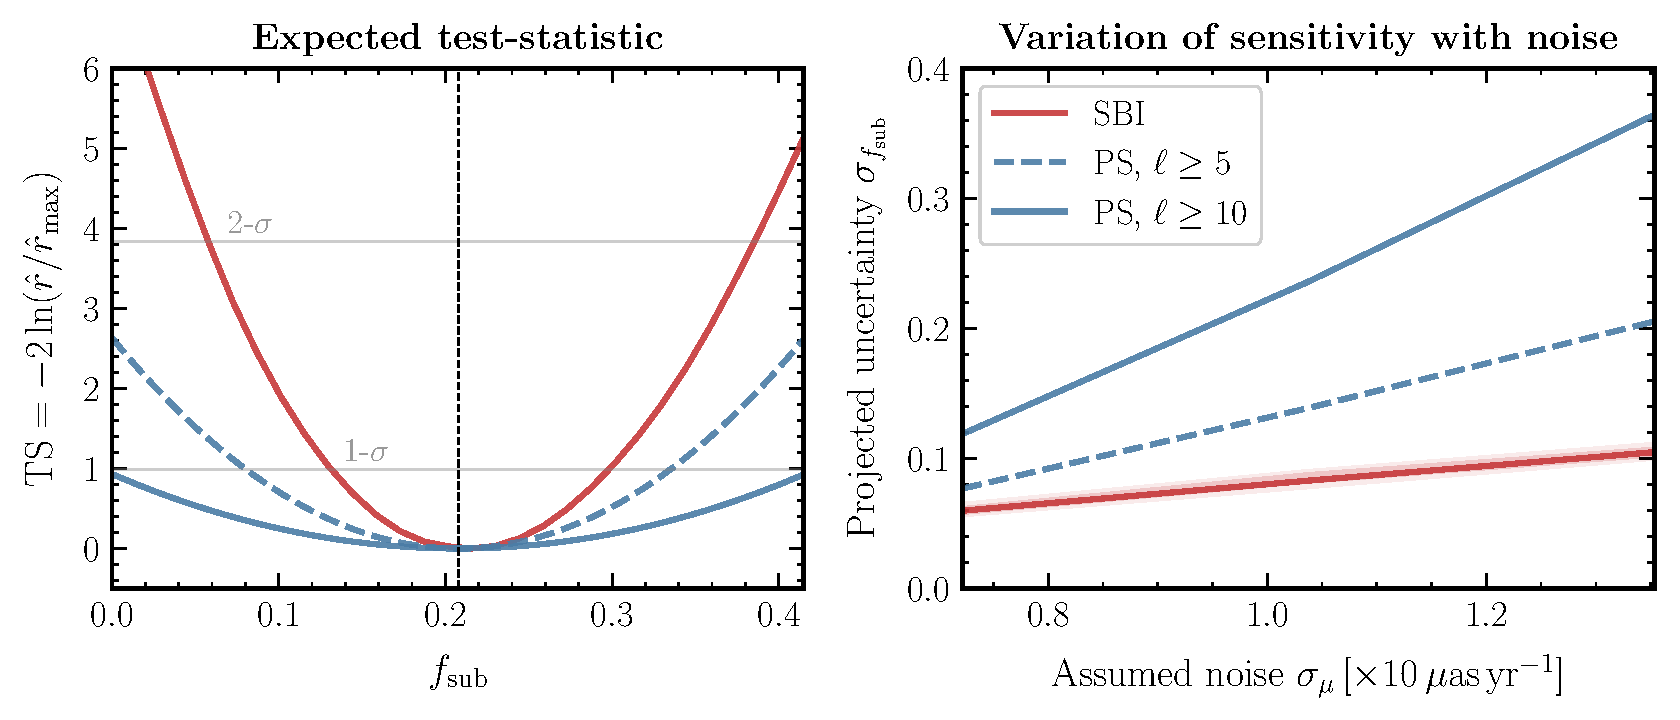
\includegraphics[width=0.99\textwidth]{figures/results}
\caption{\emph{(Left)} The expected test-statistic profile for a cold dark matter population as a function of substructure fraction $f_\mathrm{sub}$ obtained using the neural likelihood-ratio estimation method introduced in this work (red line) compared with the corresponding profiles for existing approaches using power spectrum summaries with different multipole thresholds $\ell \gtrsim 5$ (dashed blue line) and $\ell \gtrsim 10$ (solid blue line). The vertical dotted line indicates the true benchmark value of the parameter $f_\mathrm{sub}$ in the test dataset. Our method shows enhanced sensitivity to a cold dark matter population compared to traditional approaches. \emph{(Right)} Scaling of the expected sensitivities, quantified by the respective 1-$\sigma$ uncertainties, with per-object instrumental noise. For the machine learning-based approach, the band quantifies the 95\% highest-density interval on the inferred 1-$\sigma$ uncertainty. Our method shows a more favorable scaling with assumed measurement noise.}
\label{fig:experiment}
\end{figure}
 
% \begin{figure}[!htbp]
% \centering
% 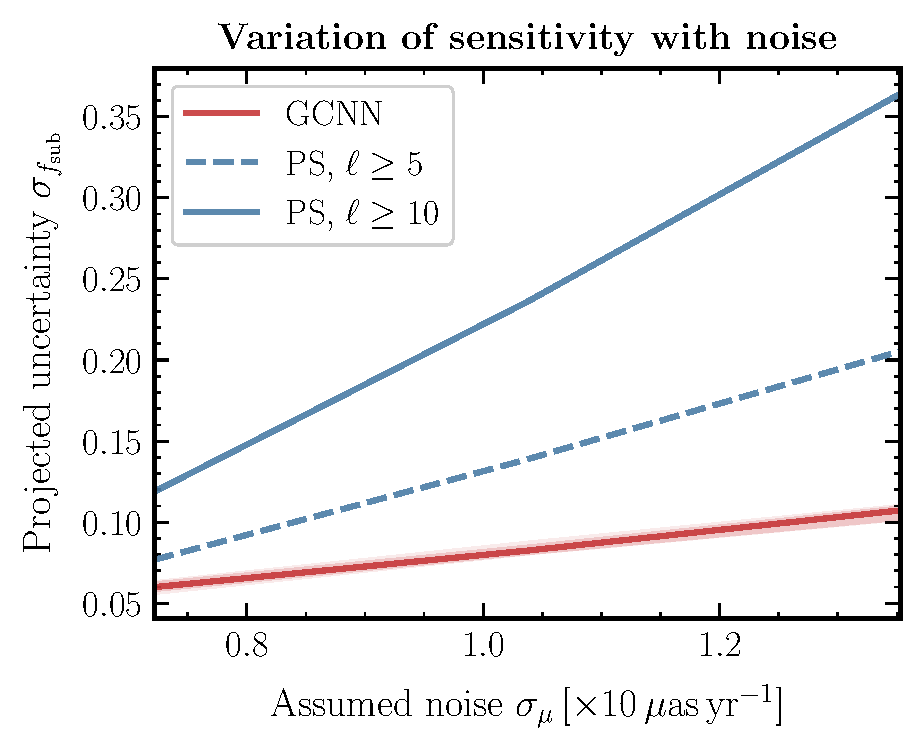
\includegraphics[width=0.49\textwidth]{figures/noise_var}
% \caption{Caption}
% \label{fig:experiment}
% \end{figure}

\section{Experiments on simulated data}
\label{sec:experiments}

\paragraph{Test-statistic profile for benchmark scenario} We evaluate our trained likelihood-ratio estimator on maps drawn from a benchmark configuration motivated by Refs.~\cite{Hutten:2016jko,Springel:2008cc}, containing 150 subhalos in expectation between $10^{8}$--$10^{10}\,\mathrm{M}_\odot$ corresponding to $f_\mathrm{sub} \simeq 0.2$. The left panel of Fig.~\ref{fig:experiment} shows the expected test-statistic (TS), defined as $\mathrm{TS} \equiv -2\ln(\hat r / \hat r_\mathrm{max})$ where $\hat r_\mathrm{max}$ is the maximum likelihood-ratio estimate in the parameter range considered, as a function of substructure fraction $f_\mathrm{sub}$ for the benchmark configuration with $f_\mathrm{sub} \simeq 0.2$. This is obtained by evaluating the trained estimator on 100 test maps over a uniform grid in $f_\mathrm{sub}$ and taking the point-wise mean. Corresponding curves using the power spectrum approach are shown in blue, using minimum multipoles of $\ell \geq 5$ (dashed) and $\ell \geq 10$ (solid). Thresholds corresponding to 1- and 2-$\sigma$ significance assuming a $\chi^2$-distributed TS are shown as the horizontal grey lines. We see that sensitivity gains of over a factor of $\sim 2$ can be expected for this particular benchmark when using the machine learning approach compared to the traditional power spectrum approach. No significant bias on the central value of the inferred DM abundance relative to the overall uncertainty scale is observed.

\paragraph{Scaling of projected uncertainty with measurement noise} The right panel of Fig.~\ref{fig:experiment} shows the scaling of expected 1-$\sigma$ uncertainty on substructure fraction $f_\mathrm{sub}$ with assumed noise per quasar, keeping the number of quasars fixed (red, with the line showing the median and shaded band corresponding to the 95\% highest-density interval on the uncertainty inferred over 50 test datasets) compared to the power spectrum approach (blue lines). A far more favorable scaling of the machine learning approach is seen compared to the power spectrum approach, suggesting that it is especially advantageous in low signal-to-noise regimes that are generally most relevant for dark matter searches.


\paragraph{Effect of correlated, unmodeled noise} Since the existence of measurement noise correlated on large spatial scales is a potential source of systematic uncertainty, we test the susceptibility of our method to such effects by creating simulated data containing large-scale noise not previously seen by the trained estimator. Instead of assuming a scale-invariant noise power spectrum $C_\ell^\mathrm{noise} = 4\pi \sigma_{\mu}^2 / N_q$~\cite{Mishra-Sharma:2020ynk}, in this case we model noise with an order of magnitude excess in power on scales $\ell \lesssim 10$ parameterized as $C_\ell^\mathrm{noise} = 4\pi\sigma_{\mu}^2 / N_q \cdot \left(10 - 9 S(\ell - 10)\right)$ where $S$ is the sigmoid function.
The left panel of Fig.~\ref{fig:noise_test} illustrates this noise model (thicker green line), as well the power spectrum of one simulated realization (thinner green line, obtained using the \texttt{HEALPix} module \texttt{anafast}) contrasted with the standard scale-invariant noise case (red lines). The right panel of Fig.~\ref{fig:noise_test} shows the expected test-statistic profile for the two cases. Although a bias in the maximum-likelihood estimate of $f_\mathrm{sub}$ is seen when the test data has unmodeled noise (green line), the true test parameter value (dashed vertical line) is seen to lie well within the inferred 1-$\sigma$ confidence interval. This suggests that the method is only marginally susceptible to substantive amounts of correlated noise on large spatial scales.

\begin{figure}[!htbp]
\centering
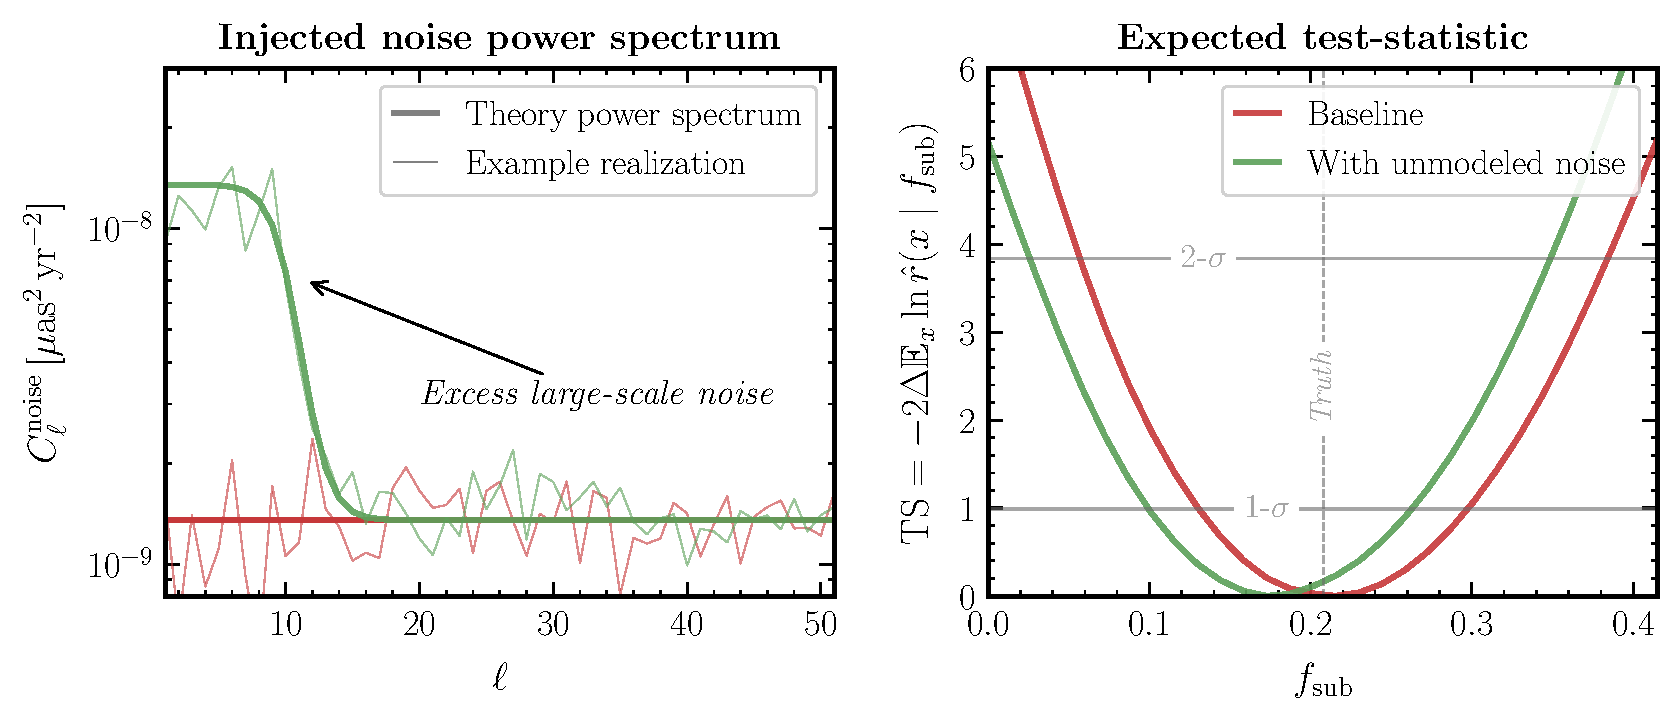
\includegraphics[width=0.99\textwidth]{figures/lowell_noise}
\caption{\emph{(Left)} The power spectrum of the noise model (thicker green line) used to study the impact of correlated noise on large spatial scales, not modeled during training, on the performance of the model. The thinner green line shows the power spectrum of an example noise realization instantiated using this noise model. The red lines show corresponding power spectra for a scale-invariant noise model.  \emph{(Right)} The expected  test-statistic profile for a model evaluated on maps containing excess large-scale noise (green line) compared to the model evaluated on maps with scale-invariant noise (red line). A small bias in the maximum-likelihood estimate returned by the model is seen when unaccounted-for noise is presented in the test maps.}
\label{fig:noise_test}
\end{figure}

\section{Conclusions and outlook}
\label{sec:conclusions}

We have introduced a method to analyze astrometric datasets over large regions of the sky using techniques based on machine learning with the aim of inferring the lensing signature of a dark matter subhalo population. We have shown our method to be significantly more sensitive to a cold dark matter subhalo population compared to established methods based on global summary statistics, with more favorable scaling as a function of measurement noise. Since the collection and reduction of astrometric data is an expensive endeavor, the use of methods that can take advantage of more of the available information can be equated to long periods of observation, underscoring their importance. Additionally, unlike the power spectrum approach, the current method does not require the construction of a numerically-expensive estimator to account for non-uniform exposure and instrumental noise in realistic datasets. These, as well as any other modeled observational effects, can be incorporated directly at the level of the forward model. 

We have focused in this work on assessing sensitivity to a cold dark matter-like subhalo population with quasar velocity astrometry, which is within the scope of upcoming radio telescopes like the SKA~\cite{Fomalont:2004hr,Jarvis:2015tqa}. Our method can also be applied in a straightforward manner to look for the \emph{acceleration} lensing signal imprinted on Milky Way stars, in particular sourced by a population of more compact subhalos than those expected in the cold dark matter scenario. Both of these features are expected to introduce a larger degree of non-Gaussianity than in the signal explored here (as can be seen, \emph{e.g.}, from Fig. 1 of Ref.~\cite{Mishra-Sharma:2020ynk}). Such analyses using Milky Way stellar accelerations is within purview of the upcoming Roman exoplanet microlensing survey~\cite{Pardo:2021uzy} as well as future \emph{Gaia} data releases, and a machine learning approach could provide significant sensitivity gains over existing methods.

Several improvements and extensions to the method presented in this paper are possible. The use of architectures that can equivariantly handle vector inputs~\cite{esteves2020spinweighted} can aid in learning more efficient representations of the astrometric map. Using convolutions based on fixed rather than learned filters can additionally reduce model complexity and produce more interpretable representations~\cite{Cheng:2020qbx,2021arXiv210709145H,2021arXiv210411244S,2021arXiv210202828M,Valogiannis:2021chp}. The use of methods for likelihood-ratio estimation that can leverage additional latent information in the forward model can significantly enhance the sample efficiency of the analysis~\cite{Brehmer:2018eca,Brehmer:2018hga,Brehmer:2018kdj,Stoye:2018ovl}. We leave the study of these extensions as well as application of our method to other dark matter population scenarios to future work.

Astrometric lensing has been established as a promising way to characterize the Galactic dark matter population, with theoretical progress in recent years going in step with advances on the observational front. While this work is a first attempt at bringing principled machine learning techniques to this field, with the availability of increasingly complex datasets we expect machine learning to be an important general-purpose tool for future astrometric dark matter searches.

Code used for reproducing the results presented in this paper is available at \url{https://github.com/smsharma/neural-global-astrometry}. 

\begin{ack}
SM warmly thanks Cristina Mondino, Tess Smidt, Ken Van Tilburg, and Neal Weiner for helpful conversations. SM benefitted from the hospitality of the Center for Computational Astrophysics at the Flatiron Institute while this work was being performed. 
This work was performed in part at the Aspen Center for Physics, which is supported by National Science Foundation grant PHY-1607611.
The participation of SM at the Aspen Center for Physics was supported by the Simons Foundation.
This work is supported by the NSF CAREER grant PHY-1554858, NSF grants PHY-1620727 and PHY-1915409, and the Simons Foundation. 
This work is supported by the National Science Foundation under Cooperative Agreement PHY-2019786 (The NSF AI Institute for Artificial Intelligence and Fundamental Interactions, \url{http://iaifi.org/}).
This material is based upon work supported by the U.S. Department of Energy, Office of Science, Office of High Energy Physics of U.S. Department of Energy under grant Contract Number DE-SC0012567.
This work made use of the NYU IT High Performance Computing resources, services, and staff expertise. 
This research has made use of NASA's Astrophysics Data System. 

This research made use of the Astropy~\cite{Robitaille:2013mpa,Price-Whelan:2018hus},
Healpy~\cite{Gorski:2004by,Zonca2019},
IPython~\cite{PER-GRA:2007},
Jupyter~\cite{Kluyver2016JupyterN},
Matplotlib~\cite{Hunter:2007},
MLflow~\cite{chen2020developments},
NumPy~\cite{harris_array_2020},
PyGSP~\cite{michael_defferrard_2017_1003158},
PyTorch~\cite{NEURIPS2019_9015},
PyTorch Geometric~\cite{Fey/Lenssen/2019}, 
PyTorch Lightning~\cite{william_falcon_2020_3828935},
sbi~\cite{tejero-cantero2020sbi},
SciPy~\cite{2020SciPy-NMeth}, and
Seaborn~\cite{michael_waskom_2017_883859}
software packages.
We acknowledge the use of the \texttt{DeepSphere} graph convolutional layer implementation as well as code used to produce elements of Fig.~\ref{fig:model} from the code repository associated with Ref.~\cite{defferrard2020deepsphere}.\footnote{\url{https://github.com/deepsphere/deepsphere-pytorch}}
\end{ack}

\bibliographystyle{apsrev4-1-mod}

{
\small
\bibliography{astrometry-sbi}
}

% %%%%%%%%%%%%%%%%%%%%%%%%%%%%%%%%%%%%%%%%%%%%%%%%%%%%%%%%%%%%
% \section*{Checklist}

% \begin{enumerate}

% \item For all authors...
% \begin{enumerate}
%   \item Do the main claims made in the abstract and introduction accurately reflect the paper's contributions and scope?
%     \answerYes{}
%   \item Did you describe the limitations of your work?
%     \answerYes{See Sec.~\ref{sec:conclusions}}
%   \item Did you discuss any potential negative societal impacts of your work?
%     \answerNA{Potential negative societal impacts were considered, and we believe this work does not present any issues in this regard.}
%   \item Have you read the ethics review guidelines and ensured that your paper conforms to them?
%     \answerYes{}
% \end{enumerate}

% \item If you are including theoretical results...
% \begin{enumerate}
%   \item Did you state the full set of assumptions of all theoretical results?
%     \answerNA{No theoretical results were obtained in this work.}
% 	\item Did you include complete proofs of all theoretical results?
%     \answerNA{}
% \end{enumerate}

% \item If you ran experiments...
% \begin{enumerate}
%   \item Did you include the code, data, and instructions needed to reproduce the main experimental results (either in the supplemental material or as a URL)?
%     \answerYes{The code repository associated with this paper and needed to reproduce all the results is linked in Sec.~\ref{sec:conclusions}.}
%   \item Did you specify all the training details (e.g., data splits, hyperparameters, how they were chosen)?
%     \answerYes{These are described in Sec.~\ref{sec:experiments}.}
% 	\item Did you report error bars (e.g., with respect to the random seed after running experiments multiple times)?
%     \answerYes{The main results in Fig.~\ref{fig:experiment} show the expectation evaluated over multiple test datasets. The right panel specifically shows the error bars associated with running over different trials.}
% 	\item Did you include the total amount of compute and the type of resources used (e.g., type of GPUs, internal cluster, or cloud provider)?
%     \answerNo{Due to space constraints limiting the total length of the extended abstract to 4 pages, this information will be included in the camera-ready version of the paper.}
% \end{enumerate}

% \item If you are using existing assets (e.g., code, data, models) or curating/releasing new assets...
% \begin{enumerate}
%   \item If your work uses existing assets, did you cite the creators?
%     \answerYes{All code used for this project is cited in the Acknowledgments section, which is redacted during blind review. Code citations will be reinstated for the camera-ready version of the paper.} 
%   \item Did you mention the license of the assets?
%     \answerNA{Licenses are mentioned in the links associated with individual code packages.}
%   \item Did you include any new assets either in the supplemental material or as a URL?
%     \answerNA{No new assets (excluding the code used to reproduced the experiments) were produced in this work.}
%   \item Did you discuss whether and how consent was obtained from people whose data you're using/curating?
%     \answerNA{}
%   \item Did you discuss whether the data you are using/curating contains personally identifiable information or offensive content?
%     \answerNA{No personal information is included in the assets utilized in this paper.}
% \end{enumerate}

% \item If you used crowdsourcing or conducted research with human subjects...
% \begin{enumerate}
%   \item Did you include the full text of instructions given to participants and screenshots, if applicable?
%     \answerNA{}
%   \item Did you describe any potential participant risks, with links to Institutional Review Board (IRB) approvals, if applicable?
%     \answerNA{}
%   \item Did you include the estimated hourly wage paid to participants and the total amount spent on participant compensation?
%     \answerNA{}
% \end{enumerate}

% \end{enumerate}

%%%%%%%%%%%%%%%%%%%%%%%%%%%%%%%%%%%%%%%%%%%%%%%%%%%%%%%%%%%%

\end{document}